\documentclass[a4paper,twocolumn,10pt]{ltjsarticle}
\usepackage[top=8mm,bottom=9mm,left=9mm,right=9mm,columnsep=6mm]{geometry}
\usepackage{amsmath,amssymb}
\usepackage{graphicx}
\usepackage{booktabs}
\usepackage{tabularx}
\usepackage{siunitx}
\usepackage{listings}
\usepackage{xcolor}
\usepackage[hidelinks]{hyperref}
\usepackage{enumitem}
\usepackage{caption}
\usepackage{subcaption}
\usepackage{titlesec}
\captionsetup{font=small,skip=2pt}
\setlist{itemsep=0pt,topsep=1pt,parsep=0pt,leftmargin=1.1em}
\titleformat{\section}{\large\bfseries\sffamily}{\thesection}{0.5em}{}
\titlespacing*{\section}{0pt}{5pt plus 1pt}{2pt}
\titleformat{\subsection}{\normalsize\bfseries\sffamily}{\thesubsection}{0.5em}{}
\titlespacing*{\subsection}{0pt}{3pt plus 1pt}{1pt}
\sisetup{detect-all}
\pagestyle{empty}
\setlength{\parskip}{0pt}
\setlength{\textfloatsep}{6pt plus 2pt minus 2pt}
\setlength{\floatsep}{4pt plus 1pt minus 1pt}
\setlength{\dbltextfloatsep}{6pt plus 2pt minus 2pt}
\setlength{\intextsep}{4pt plus 1pt minus 1pt}
\newcommand{\figref}[1]{図~\ref{#1}}
\newcommand{\tabref}[1]{表~\ref{#1}}
\newcommand{\lstref}[1]{リスト~\ref{#1}}
\newcommand{\code}[1]{\texttt{#1}}

\definecolor{lstbg}{gray}{0.955}
\lstset{
  basicstyle=\ttfamily\fontsize{6.3}{7.3}\selectfont,
  backgroundcolor=\color{lstbg}, frame=single, rulecolor=\color{gray!60},
  breaklines=true, columns=fullflexible, keepspaces=true,
  xleftmargin=1pt, xrightmargin=1pt, aboveskip=3pt, belowskip=3pt,
  framesep=2pt
}
\renewcommand{\lstlistingname}{リスト}


% Match Latin and Japanese heading glyphs to the same font file.
\usepackage{luatexja-fontspec}
\setsansfont{HaranoAjiGothic-Medium.otf}[BoldFont=HaranoAjiGothic-Medium.otf]
\setsansjfont{HaranoAjiGothic-Medium.otf}[BoldFont=HaranoAjiGothic-Medium.otf]














\usepackage{multicol}





\begin{document}\onecolumn

\begin{center}{\LARGE\bfseries\sffamily ロボコンの無線通信と帯域共有の実測評価\par}
\vspace{1mm}{\normalsize 他チーム通信・ROS 2・Bluetooth・ESP-NOW\par}
\vspace{.5mm}{\normalsize 貝淵蒼馬\par}\end{center}
\noindent\fbox{\parbox{\dimexpr\textwidth-2\fboxsep-2\fboxrule}{\small
\textbf{要旨}\quad 指令と大容量データを同時に流し、他チームの通信、チャネル幅、QoS、指令周期を比較した。
実測SDR画像は帯域の重なりを示す。一方、指令が期限内に届くかはアプリの応答記録から評価する。
チャネルを分離しても端末内部や同じチーム内の遅延は残り、帯域幅・平均速度・接続表示だけでは操縦品質を判断できなかった。}}\vspace{2mm}
\begin{multicols}{2}
\section{目的と実験方法}
スマートフォンからの指令、カメラ映像、LiDAR点群を同じWi-FiとROS 2で運ぶロボットを想定する。
自チーム内だけでなく、隣のチームも大容量通信中の条件を作った。
観測PC（Intel BE200）がCh6・20 MHz AP、ラップトップ2（MT7921E）がロボット役、
ラップトップ1（Intel AX210）が有線でインターネットを共有する。
ESP32 3台は指令、別チームAP／STA、独立BLE、ESP-NOWへ順次使用した。

先行試験は64 byte・100 Hz UDP指令とTCP模擬データをSTA→AP→STAへ通した。
追加の実ROS 2試験はPC AP→STA（指令側Humble・ロボット側Jazzy、双方CycloneDDS）、ImageとPointCloud2を各10 Hzで生成する。
合成センサの要求payloadは60.54 Mbps、実受信は約47--55 Mbpsだった。
実カメラ、スマートフォン、モータは使用していない。経路の異なる系列を混ぜて方式の順位を決めない。

1試行30秒・3反復を基本とし、ESP-NOW長時間系列だけ600秒・2--3反復とする。
RTT p99は応答が戻った指令の分位点、20 ms期限超過率は\textbf{全予定指令が分母で欠落も含む}。
最新sequenceの更新途絶も評価する。20 msは比較目標で、ロボットの安全限界ではない。
環境の反復数はパケット数とは区別する。

\section{他チーム通信とチャネル配置}
\begin{center}\captionof{table}{自チーム大容量TCP中。値は他チーム待機／負荷。各3反復。}
\small\begin{tabular}{@{}crr@{}}\toprule 他Ch & RTT p99 [ms] & 20 ms超過 [\%]\\\midrule
6 & 125.8 / 148.4 & 55.0 / 67.7\\
7 & 123.8 / 132.3 & 53.8 / 63.0\\
11 & 126.5 / 127.4 & 54.4 / 57.2\\
\bottomrule\end{tabular}\end{center}
他チームを負荷へ変えると、p99の増分は同一Ch6で約23 ms、隣接Ch7で約9 ms、分離Ch11で約1 msだった。
\textbf{別のチャネル番号でも帯域が分かれるとは限らない}。Ch6とCh7は中心が5 MHzしか離れず、20 MHz幅で大きく重なる。
同一Chが今回最も遅く、隣接が常に最悪という結果ではない。

同一帯域の送信待ち、部分重複による受信妨害、再送などが候補になる\cite{rf}。
再送数やキャリアセンスを直接測っておらず、色だけで原因を特定しない。
他チーム実受信量も約0.4--4.7 Mbpsと異なるため、等しい干渉電力や空中時間の比較ではない。

\subsection{チャネル幅と周波数の余裕}
Ch1の20 MHzは名目上2402--2422 MHz、Ch6は2427--2447 MHz。
Ch1＋副Ch5の40 MHzでは約2402--2442 MHzとなりCh6へ重なる。
20→40 MHzでp99は128.6→127.5 ms、期限超過は55.0→56.8\%だった。
帯域が広いほど同時配置の余裕は減るが、転送が速くなれば同じデータの送信時間は短くなる。
\textbf{広いほど必ず悪いとは言えず、実受信量と指令期限を併せて判断する}。
今回の幅比較は他チームAPの介入で、自チームAPの最高速度比較ではない。

\subsection{基準性能の確認}
操縦のみ・他待機でもUDPのp99は117--120 ms、20 ms超過は47--49\%だった。
既に目標を満たさない構成なので、全遅延を他チームへ帰属しない。
RTTを2で割って片道値にすることや、別PC時計の差を未同期で使うことはできない。
\end{multicols}
\begin{center}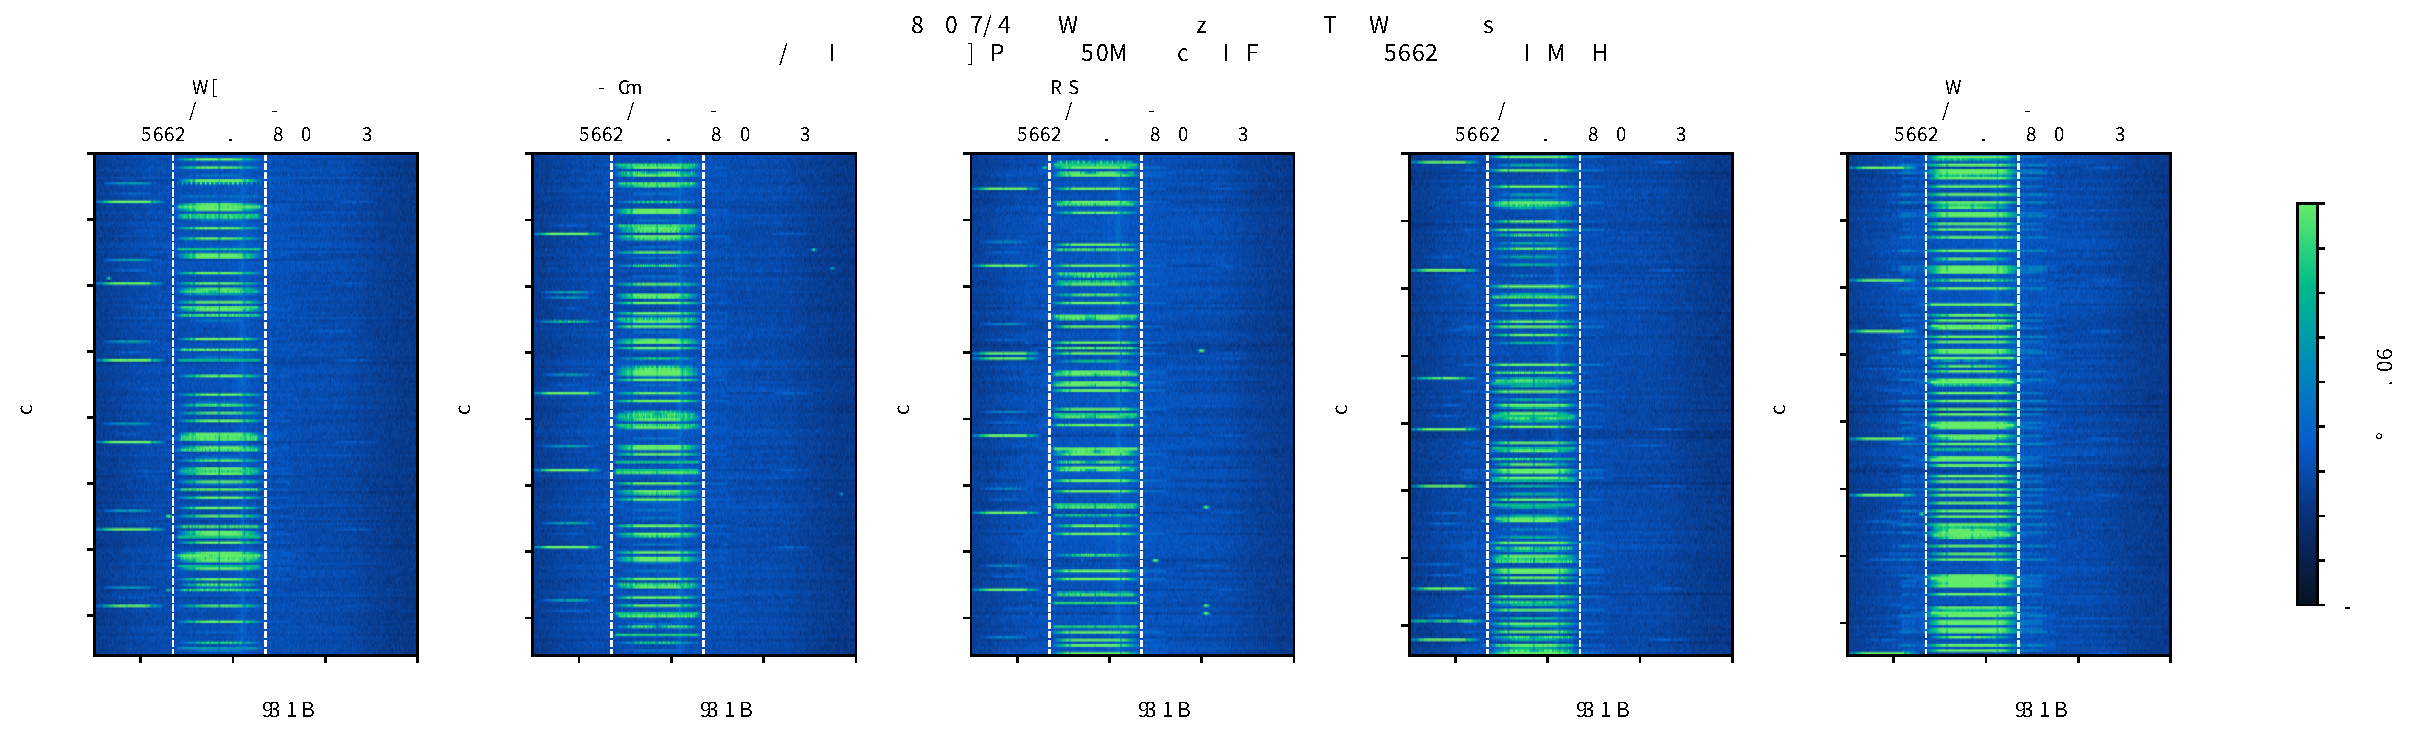
\includegraphics[width=.95\textwidth]{../experiments/figures/operational/placement-blue-green.pdf}\captionof{figure}{短い配置比較のWi-Fi負荷・反復1。中心間距離とC5までの距離を併記。共通ゲイン・未校正dBFS。}\end{center}
\clearpage

\begin{center}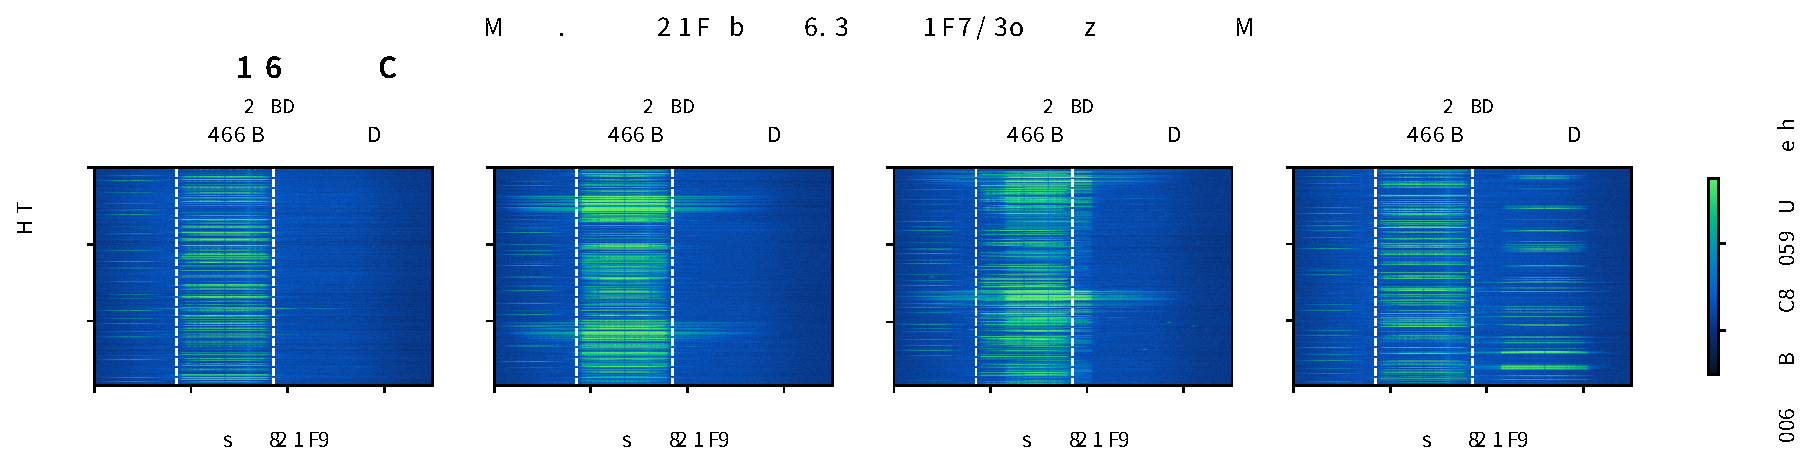
\includegraphics[width=.98\textwidth]{../experiments/figures/two-team/two-team-blue-green-compact.pdf}\captionof{figure}{自チームCh6で指令＋大容量通信。他チーム負荷を同一・隣接・分離へ変更。反復1、共通ゲインと色尺度。}\end{center}
\begin{multicols}{2}
\section{流量・生成周期・ROS 2の比較}
追加の流量試験では他チームを負荷中に固定し、自チームTCPの要求量を0--2 Mbpsへ変えた。
同一Ch6の0→1 Mbpsで20 ms超過は54.08→72.61\%、実受信平均は1.007 Mbpsだった。
2 Mbps要求でも実受信は1.105 Mbpsにとどまり、生成byteが未送信で積み上がった。
\textbf{設定Mbpsを達成速度や無線負荷とみなさず、生成・送信受付・実受信を分ける}。

同じ1 Mbps要求で生成周期100→10 msへ変えると、Ch6の超過は63.47→59.42\%だったが、
Ch7では53.88→53.88\%だった。小分け生成は常に改善する結果ではなく、TCPやOSはbyteをまとめ直せる。
平均量に加え時間的な集中と端末の待ち行列を評価する必要がある。

\subsection{QoSと大容量トピック}
指令QoSはreliable・深さ10に固定し、センサだけbest effort／reliable、深さ1／10を比較した。
指令のみの20 ms超過は約45\%、センサ追加時は約70--80\%となった。
best effort・深さ1でも同一Ch6のp99は145.57 ms、超過77.68\%だった。
深さ1はDDSの履歴設定であり、無線待ち行列を1つにしたり指令を優先したりする設定ではない\cite{ros}。
画像のunique sequence初回受信間隔には最大3.33秒の途絶もあった。
受信間隔は観測できたが、生成から到着までのデータの古さは未同期時計から計算していない。

\subsection{省電力と遅延の切り分け}
端末の省電力ON／OFFを実際に切り替え、前後のreadbackを確認した。
指令のみでは両方p99約103--109 msが残った。一方センサ負荷・他Ch11ではOFF→ONで163.38→248.66 msだった。
省電力OFFだけで今回の遅延は解消しない。
予定送信のずれは約0.5--1 ms、publish呼出し約0.08 ms、ロボット内の応答前処理約0.003--0.007 msだった。
publishが速くても、その後のDDS・OS・MACの待ちは残る。p99を引き算して原因の寄与を割り当てない。

\section{SDR画像の読み方}
C5：80 MS/s、16,380 I/Q、アナログ帯域48 MHz、ゲイン20、FFT1024。
各行約205 $\mu$s、名目RF観測時間比約0.4\%であり、縦軸は\textbf{間欠取得順}。
青緑は未校正dBFSで、同じ図の共通尺度内で比較する。
緑の割合を占有率、通信成功率、絶対dBmへ換算しない。
Ch11の一部は名目アナログ帯域の端へかかり、弱い色を無干渉の証拠としない。
画像で帯域の重複、アプリ記録で届く時刻、実受信量で負荷の実現度を確かめる。
\end{multicols}
\clearpage

\begin{center}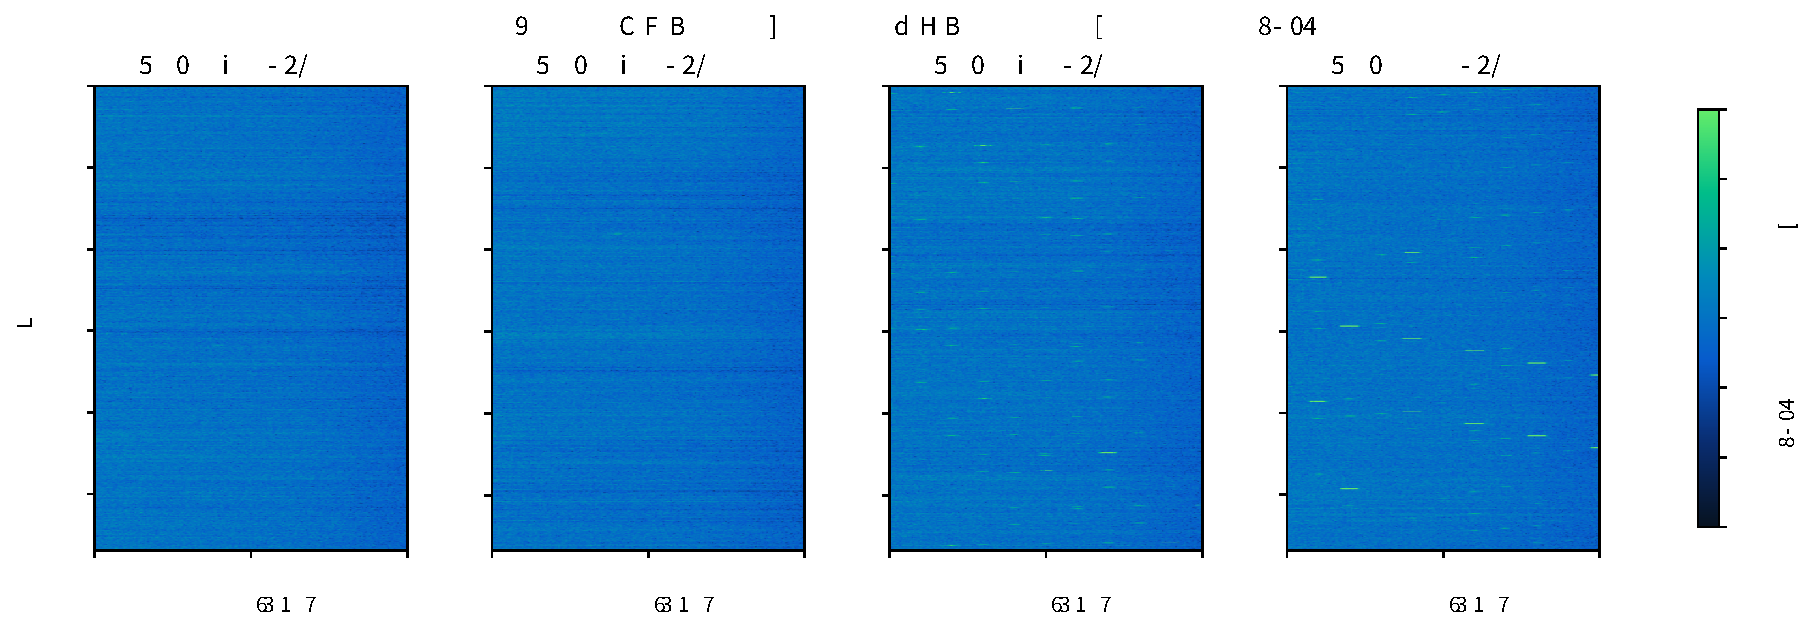
\includegraphics[width=.91\textwidth]{../experiments/figures/two-team/ble-narrow-blue-green.pdf}\captionof{figure}{BLE停止・広告・GATT通知。2450--2470 MHzの拡大、反復1。この図は−90〜−60 dBFSで前ページとは尺度が異なる。}\end{center}
\begin{multicols}{2}
\section{Bluetooth LEとの共存}
独立したESP32 2台でBLE停止、20 ms設定の広告、BLE 1M GATT通知を比較し、
広告の復号数と実通知受信量を確認した。Wi-Fi大容量通信中のp99は停止126.2 ms、広告126.0 ms、通知126.3 msだった。
通知の平均実受信量はWi-Fi待機0.36→負荷0.33 Mbps。
今回はBLE追加でWi-Fi p99が大きく増える結果ではないが、両リンクの配送量を評価する意義がある。
通知時の狭い成分は方式の違いを示す手掛かりであり、全ての細線をBLEと同定した結果ではない。
同一チップ内の共存、Bluetooth音声、連続ホッピングの復元は未検証である。

\section{ESP-NOW指令の周期と更新途絶}
2台間で64 byteを往復し、20・50・100・200 Hz、別系統Wi-Fi Ch6の待機／TCP負荷を各600秒測った。
使用者の終了希望で19試行（8条件、各2--3反復）とし、残り5試行は未実施。
960,000予定指令を全て送信し、959,997 unique応答を記録した。
MAC送信成功はアプリ応答やアクチュエータ動作成功とは異なる\cite{espnow}。
\begin{center}\captionof{table}{長時間系列のWi-Fi負荷条件。欠落も超過に含む。}
\small\begin{tabular}{@{}rrrr@{}}\toprule Hz & p99 [ms] & 20 ms超過 [\%] & 最大更新途絶 [ms]\\\midrule
20 & 9.18 & 0.0167 & 100.7\\
50 & 9.62 & 0.0267 & 46.5\\
100 & 9.26 & 0.0008 & 23.9\\
200 & 14.26 & 0.2108 & 36.8\\
\bottomrule\end{tabular}\end{center}
100 Hz・負荷中はp99 9.26 msだったが、200 Hzでは14.26 ms、10秒窓の超過が集中する区間もあった。
\textbf{指令周期を短くすれば必ず通信が良くなるわけではない}。
20 Hzの通常更新間隔自体が50 msであるため、1応答の20 ms期限と継続更新の周期は別に設計する。
200 Hzのpayloadは片道0.1024 Mbpsだが、ヘッダ・ACK・送信待ちも必要で空中時間とは一致しない。
旧30秒系列ではCh6負荷p99が反復8.6--123.8 msと変動した。実装・取得時間が違うので今回へ混ぜない。
Wi-Fiの実受信は約1.7--2.7 Mbps、AP中継UDP／ROS 2と無線経路も異なり、方式だけの勝敗は決められない。
\subsection{短時間の配置比較}
送受信75 cm、C5→送信45 cm、C5→応答95 cmを基準に、応答機の90°回転、手による遮蔽、送受信150 cmへの距離変更、基準復帰を各10秒・3反復で比較した。
基準前の負荷中p99は10.91 ms、超過0.000\%。
回転の負荷中p99は7.79 ms、超過0.000\%。
遮蔽の負荷中p99は7.93 ms、超過0.000\%。
距離変更の負荷中p99は8.83 ms、超過0.000\%。
基準後の負荷中p99は8.63 ms、超過0.000\%。
全30試行・30,000指令で応答欠落はなかった。基準復帰後もp99が下がったため、回転や遮蔽による改善とは断定できない。届いた最新パケットのRSSIだけで欠落時の感度は判断できない。C5までの距離、ケーブルや反射を含め、短時間の結果を到達距離の保証へ広げない。

\section{ロボコン運用への示唆}
本番前にカメラ・点群を動かし、隣のチームにも通信を流してもらい、単独基準と同条件で比較する。
チャネル分離、生成量、周期、QoS、省電力は一つずつ変え、平均速度と\textbf{期限超過・欠落・最長更新途絶}を残す。
古い指令を追いつくまで送るより、最新指令の扱いと途絶時の動作を設計する。
後者は今回モータで検証しておらず、実機の停止期限は別に確かめる必要がある。

{\footnotesize
\section{公開データと再現性}
詳細版には先行受信・5 GHz分割合成も統合し、異なる系列を区別した。
相対イベント時刻、FFT電力、匿名条件と検算・描画・取得コードを公開。元I/Q、PCAP、私有ログは非公開保管する。
保存不完了の600秒アプリ記録は補足として保持し、正式19試行へ含めない。
\url{https://github.com/Raptor-zip/esp-sdr-robotics-wifi}
\begin{thebibliography}{9}\footnotesize
\bibitem{rf} \href{https://www.cisco.com/c/en/us/td/docs/wireless/controller/9800/technical-reference/wireless-rf-reference-guide.html}{Cisco, Wireless RF Reference Guide.}
\bibitem{ros} \href{https://docs.ros.org/en/jazzy/Concepts/Intermediate/About-Quality-of-Service-Settings.html}{ROS 2 Jazzy, Quality of Service settings.}
\bibitem{espnow} \href{https://docs.espressif.com/projects/esp-idf/en/v6.0/esp32/api-reference/network/esp_now.html}{Espressif, ESP-NOW Programming Guide.}
\end{thebibliography}}
\end{multicols}
\end{document}
